% ****** Start of file apssamp.tex ******
%
%   This file is part of the APS files in the REVTeX 4.1 distribution.
%   Version 4.1r of REVTeX, August 2010
%
%   Copyright (c) 2009, 2010 The American Physical Society.
%
%   See the REVTeX 4 README file for restrictions and more information.
%
% TeX'ing this file requires that you have AMS-LaTeX 2.0 installed
% as well as the rest of the prerequisites for REVTeX 4.1
%
% See the REVTeX 4 README file
% It also requires running BibTeX. The commands are as follows:
%
%  1)  latex apssamp.tex
%  2)  bibtex apssamp
%  3)  latex apssamp.tex
%  4)  latex apssamp.tex
%
\documentclass[%
 reprint,
%superscriptaddress,
%groupedaddress,
%unsortedaddress,
%runinaddress,
%frontmatterverbose, 
%preprint,
%showpacs,preprintnumbers,
%nofootinbib,
%nobibnotes,
%bibnotes,
 amsmath,amssymb,
 aps,
%pra,
%prb,
%rmp,
%prstab,
%prstper,
%floatfix,
10.5pt,
]{revtex4-1}

\usepackage{graphicx}% Include figure files
\usepackage{subfigure}
\usepackage{multirow}
\usepackage{array}
\usepackage{dcolumn}% Align table columns on decimal point
\usepackage{bm}% bold math
%\usepackage{hyperref}% add hypertext capabilities
%\usepackage[mathlines]{lineno}% Enable numbering of text and display math
%\linenumbers\relax % Commence numbering lines

%\usepackage[showframe,%Uncomment any one of the following lines to test 
%%scale=0.7, marginratio={1:1, 2:3}, ignoreall,% default settings
%%text={7in,10in},centering,
%%margin=1.5in,
%%total={6.5in,8.75in}, top=1.2in, left=0.9in, includefoot,
%%height=10in,a5paper,hmargin={3cm,0.8in},
%]{geometry}

\usepackage{xeCJK}
%\setCJKmainfont[ItalicFont={KaiTi}, BoldFont={KaiTi}]{KaiTi}
\usepackage{textcomp}
\usepackage{chemfig}
\usepackage[version=4]{mhchem}
\usepackage{fontspec}
\usepackage{listings}
\usepackage{xcolor}
\usepackage{xcolor} % 定制颜色
\definecolor{mygreen}{rgb}{0,0.6,0}
\definecolor{mygray}{rgb}{0.5,0.5,0.5}
\definecolor{mymauve}{rgb}{0.58,0,0.82}
\lstset{
backgroundcolor=\color{white},      % choose the background color
basicstyle=\footnotesize\ttfamily,  % size of fonts used for the code
columns=fullflexible,
tabsize=4,
breaklines=true,               % automatic line breaking only at whitespace
captionpos=b,                  % sets the caption-position to bottom
commentstyle=\color{mygreen},  % comment style
escapeinside={\%*}{*)},        % if you want to add LaTeX within your code
keywordstyle=\color{blue},     % keyword style
stringstyle=\color{mymauve}\ttfamily,  % string literal style
frame=single,
rulesepcolor=\color{red!20!green!20!blue!20},
% identifierstyle=\color{red},
language=Mathematica,
}

\usepackage[normalem]{ulem}

\newcommand{\chuhao}{\fontsize{42pt}{44.9pt}\selectfont}    % 初号, 1.5倍行距
\newcommand{\xiaochu}{\fontsize{30pt}{40pt}\selectfont}    % 小初, 1.5倍行距
\newcommand{\yihao}{\fontsize{26pt}{36pt}\selectfont}    % 一号, 1.4倍行距
\newcommand{\erhao}{\fontsize{22pt}{28pt}\selectfont}    % 二号, 1.25倍行距
\newcommand{\xiaoer}{\fontsize{18pt}{18pt}\selectfont}    % 小二, 单倍行距
\newcommand{\sanhao}{\fontsize{16pt}{24pt}\selectfont}    % 三号, 1.5倍行距
\newcommand{\xiaosan}{\fontsize{15pt}{22pt}\selectfont}    % 小三, 1.5倍行距
\newcommand{\sihao}{\fontsize{14pt}{21pt}\selectfont}    % 四号, 1.5倍行距
\newcommand{\sihaox}{\fontsize{14pt}{28pt}\selectfont}    % 四号, 1.5倍行距
\newcommand{\banxiaosi}{\fontsize{13pt}{19.5pt}\selectfont}    % 半小四, 1.5倍行距
\newcommand{\xiaosix}{\fontsize{12pt}{24pt}\selectfont} 	% 小四, 1.5倍行距
\newcommand{\xiaosi}{\fontsize{12pt}{18pt}\selectfont}     
\newcommand{\dawuhao}{\fontsize{11pt}{11pt}\selectfont}    % 大五号, 单倍行距
\newcommand{\wuhao}{\fontsize{10.5pt}{10.5pt}\selectfont}    % 五号, 单倍行距
\newcommand{\xiaowu}{\fontsize{9pt}{9pt}\selectfont}    % 五号, 单倍行距

%\usepackage[fntef]{ctexcap}
%\CTEXsetup[number={\chinese{section}、},format={\Large\bfseries}]{section}
%\setCJKfamilyfont{fangsong}{FangSong}                      %仿宋2312 fs  
%\newcommand{\fangsong}{\CJKfamily{fangsong}}  

\usepackage{wrapfig}
\usepackage{fancyhdr}
\usepackage{fancybox}   


\usepackage{tikz}
\usepackage{circuitikz}



\newcommand{\bra}[1]{\langle #1 |}
\newcommand{\ket}[1]{| #1 \rangle}
\newcommand{\bracket}[2]{\langle #1 | #2 \rangle}
\newcommand{\bracketl}[3]{\langle #1 | #2 | #3 \rangle}
\newcommand{\func}{\mathrm \,}
\newcommand{\define}[2]{
	\begin{definition}
	\begin{description}
	\item[#1]
	#2
	\end{description}
	\end{definition}
}

\newcommand{\sch}{Schr\"odinger}
\newcommand{\grad}{\nabla}
\newcommand{\ueq}{\neq}
\newcommand{\celsius}{\ensuremath{^\circ\hspace{-0.09em}\mathrm{C}}}
\newcommand{\unit}[2]{$#1 \, \mathrm{#2}$}

\begin{document}

%\preprint{APS/123-QED}

\title{Measurement of the rate constant and the activation energy of ethyl acetate saponification}% Force line breaks with \\
%\thanks{A footnote to the article title}% give thanks

\author{Rui Li}
 %\altaffiliation[Also at ]{Physics Department, XYZ University.}%Lines break automatically or can be forced with \\
%\author{Second Author}%
%\email{3160102098@zju.edu.cn}
\affiliation{%
 Qiushi science class (chemistry)\\
 Chu Kochen Honor College
}%

%\collaboration{MUSO Collaboration}%\noaffiliation

%\author{Zong Wei Huang}
% \homepage{http://www.Second.institution.edu/~Charlie.Author}
%\affiliation{
% Second institution and/or address\\
% This line break forced% with \\
%}%
%\affiliation{
%Qiushi science class (chemistry)\\
% Chu Kochen Honor College
%}%
%\author{Delta Author}
%\affiliation{%
% Authors' institution and/or address\\
% This line break forced with \textbackslash\textbackslash
%}%

%\collaboration{CLEO Collaboration}%\noaffiliation

%\date{\today}% It is always \today, today,
             %  but any date may be explicitly specified

%\pacs{Valid PACS appear here}% PACS, the Physics and Astronomy
                             % Classification Scheme.
%\keywords{Suggested keywords}%Use showkeys class option if keyword
                              %display desired
\maketitle
\begin{figure*}[h]
\centering
\subfigure[Fitted curve]{
	\includegraphics[width=0.36\textheight]{figures/soapdynamics.eps}
}
\subfigure[$\ln{k}-\frac{1}{T}$]{
	\includegraphics[width=0.3\textheight]{figures/SoapArrhenius.eps}
}
\caption{The fitted curve of the reaction process with a fit of $k$ according to Arrhenius equation}
\end{figure*}
\begin{figure*}
\centering
\subfigure[distribution]{
	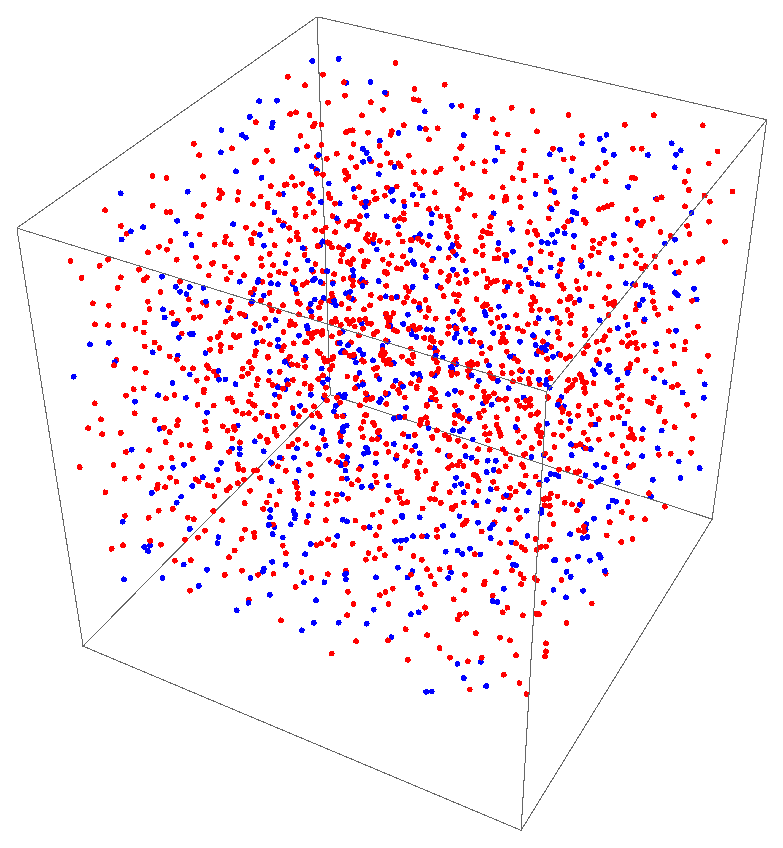
\includegraphics[width=0.4\textwidth]{figures/MeOHH2Odistribution.eps}
}
\subfigure[density plot]{
	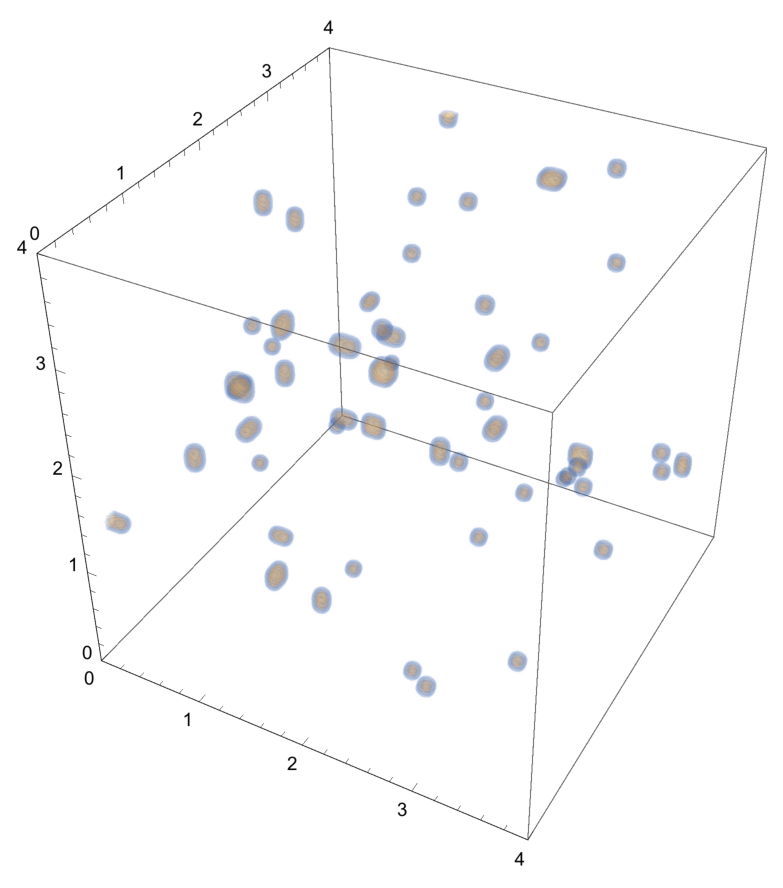
\includegraphics[width=0.4\textwidth]{figures/fuck.eps}
}
\caption{The distribution of MeOH-\ce{H2O} mixed system with molar ratio of 3:7. Red dots in the first figure stands for the position of \ce{H2O}, while the stains in the second figure stands for the clusters of MeOH molecules.}
\label{MeOH}
\end{figure*}
\begin{table}
\caption{The fitting result of the reaction rate constant}
\begin{tabular}{|c|c|c|c|c|c|c|}\hline
$T$/\celsius & \multicolumn{2}{c|}{25} & 30 & 35 & 40 & 45 \\\hline
$k$ & 0.09517 & 0.08650 & 0.1423 & 0.1609 & 0.2445 & 0.3392 \\\hline
\end{tabular}
\label{data}
\end{table}
Starting from
\begin{equation}
	E_t = \frac{1}{ak}\frac{E_0-E_t}{t} + E_\infty
\end{equation}
It is deduced that
\begin{equation}
	E_t = \frac{E_0 + ak E_\infty t}{1+ a k t}
\end{equation}
Thanks to machine learning integrated in \emph{Mathematica}, the coefficients can be derived out immediately:
\begin{lstlisting}
In[377]:= c1 /. (NonlinearModelFit[#, (-c2 + c1 c3 t)/(
      1 + c1 t), {c1, c2, c3}, t][
     "BestFitParameters"] & /@ (Transpose[{Range[Length[#]] + 
         1, #}] & /@ react))

Out[377]= {0.000951675, 0.000865023, 0.00142327, 0.0016089, \
0.0024449, 0.00339182}
\end{lstlisting}
which is equivalent to the result shown in Table.\ref{data}. The arrhenius fitting result is
\begin{equation}
	k = 13.8186 - \frac{6211.05}{T/\mathrm{K}} 
\end{equation}
giving $E_a$ = 51.64 kJ/mol, which is much larger than that from the reference ($41.4\pm 0.6 \, \mathrm{kJ/mol}$)\cite{soap}. This might result from the remainder of NaOH solution in the tube, which cannot be eliminated by just pressing the air into the apparatus. Such a mechanism of mixing the two solutions also allow a delay before forming a complete mixture, which contributes to a deviation of the dynamic equation that truly describes the system. 

For a grand system with arbitrary concentration of two solutions,
\begin{equation}
	\frac{d x_1}{dt} = \frac{d x_2}{dt} = k x_1 x_2
\end{equation}
which has a solution according to \emph{Mathematica}
\begin{equation}
\begin{cases}
	x_2(t)\to c_1-\frac{e^{c_1 c_2} c_1}{e^{c_1 c_2}-e^{c_1 k t}} \\
	x_1(t)\to -\frac{e^{c_1 c_2} c_1}{e^{c_1 c_2}-e^{c_1 k t}}
   \end{cases}
\end{equation}
where $x_1(t),x_2(t)$ stands for the concentration of two solutions, $c_1,c_2$ being two constants. However, this solution fail to give proper solution to the system. Thus its approximation is considered, where the difference of the concentration between two solution is regarded as a constant perturbation, namely
\begin{equation}
\frac{d x}{dt} = - k x (x-\Delta x)
\end{equation}
which leads to
\begin{equation}
	x(t) = \frac{a \Delta x e^{k t \Delta x }}{a e^{k t \Delta x }-a+\Delta x}
\end{equation}
Considering that $\Delta x$ is comparatively small, the equation simplifies to
\begin{equation}
	x(t) \sim \frac{a \Delta x e^{k t \Delta x }}{k t \Delta x+\Delta x} = \frac{a}{1+ kt} e^{kt\Delta x}
\end{equation}
thus the term $e^{kt\Delta x}$ acts as a amplifier for $k$, which successfully explains the deviation of the result. 

Microscopic perspective of the system may lead to another doubt that the reaction may not completely follow the second-order mechanism. Simulation of the molecular distribution of methanol and water is well studied, as shown in Fig.\ref{MeOH}, which reveals that the methanol molecules are not uniformly distributed in the water solution. It is of quite reasonable that the ethyl acetate is suffering the same situation in the water solution, which indicates that its practical concentration is over-estimated, which leads to exaggerated rate constant, which again explains the error. 


\bibliography{References}
\end{document}
